%
%  Vincent Yannello
%
\documentclass[12pt,fullpage]{article}
\usepackage{fullpage}
\usepackage{amsmath}
\DeclareMathOperator{\erf}{erf}
\usepackage{psfrag}                                          % LaTeX graphics tool
\usepackage{pslatex}                                         % avoids the default cmr font
\usepackage{graphicx}                                        % graphics package 
\usepackage{epsfig}                                          % figures
\usepackage{hyperref}
\usepackage{color}

\begin{document}

\noindent
{\bf IDB distribution} (from \color{blue}\url{http://www.math.wm.edu/~leemis/chart/UDR/UDR.html}\color{black})

\noindent
The shorthand $X \sim {\rm IDB}(\delta, \kappa, \gamma)$ is used to indicate that the
random variable $X$ has the IDB distribution with parameters $\delta$, $\kappa$, and $\gamma$.
An IDB random variable $X$ with parameters $\delta$, $\kappa$, and $\gamma$ has probability density function 
$$
f(x) = \frac{\left(  \left( 1+{\it \kappa}\,x \right) {\it \delta}\,x+\gamma
 \right) {e^{-1/(2\,{\it \delta}\,{x}^{2})}}}{\left( 1+{\it \kappa}
\,x \right) ^{{\gamma/{\it \kappa}}+1}}\qquad \qquad x > 0,
$$
for all $\delta > 0$, $\kappa > 0$, and $\gamma \geq 0$.
The probability density function with three parameter settings is illustrated below.
{\begin{figure}[h!]
\begin{center}
\psfrag{lab1}{$\delta \kern -0.08 em = \kern -0.08 em  1,\, \gamma \kern -0.08 em  = \kern -0.08 em  2, \kappa = 10$}
\psfrag{lab2}{$\delta \kern -0.08 em  = \kern -0.08 em  2,\, \gamma \kern -0.08 em  = \kern -0.08 em  5, \kappa  \kern -0.08 em = \kern -0.08 em  1$}
\psfrag{lab3}{$\delta \kern -0.08 em  = \kern -0.08 em  2,\, \gamma \kern -0.08 em  = \kern -0.08 em  0, \kappa \kern -0.08 em  = \kern -0.08 em  1$}
\psfrag{labx}{$x$}
\psfrag{labf}{$f(x)$}
\includegraphics[width=3.2in]{IDBPlot.ps}
\end{center}
\end{figure}}\\
The cumulative distribution, survivor, hazard, 
cumulative hazard, inverse distribution, moment generating, and characteristic functions on the support 
of $X$ are mathematically intractable.\\
The population mean, variance, skewness, and kurtosis of $X$ are mathematically intractable.

\vspace{0.1in}

\noindent
{\bf APPL failure:}
The APPL statements
\begin{verbatim}
assume(delta>0);
assume(kappa>0);
assume(y>=0);
X := [[x -> ((1 + kappa * x) * delta * x + y) / ((1 + kappa * x) ^ (y / kappa + 1)) 
        * exp(-delta * x ^ 2 / 2)], [0,infinity], ["Continuous", "PDF"]];
CDF(X);
SF(X);
HF(X);
CHF(X);
IDF(X);
\end{verbatim}
fail to yield the cumulative distribution, survivor, hazard, cumulative hazard, and inverse distribution functions.

\end{document}
